\documentclass[dvipsnames]{beamer}

\usetheme{m}

\usepackage[croatian]{babel}
\usepackage{booktabs}
\usepackage{minted}

\usepackage{tikz}
\usetikzlibrary{arrows,arrows.meta,positioning,fit,shapes,calc,decorations.markings,decorations.text}
\usepackage{pgfplots}

\usepgfplotslibrary{dateplot}

\usemintedstyle{trac}

\title{Server za prijenos podataka iz postrojenja}
\subtitle{}
\date{\today}
\author{Damir Jelić}
\institute{Elektrotehnički fakultet Osijek}

\begin{document}

\maketitle

\begin{frame}[fragile]
    \frametitle{Cilj diplomskog rada}
    Cilj je diplomskog rada ispitati mogućnost korištenja jeftinih
    mikroupravljača
    za jednostavne poslove automatizacije te omogućiti udaljeno upravljanje
    postrojenjem preko \emph{socket} \emph{servera}.
\end{frame}

\begin{frame}[fragile]
\frametitle{Uvod}
\begin{figure}[H]
\centering
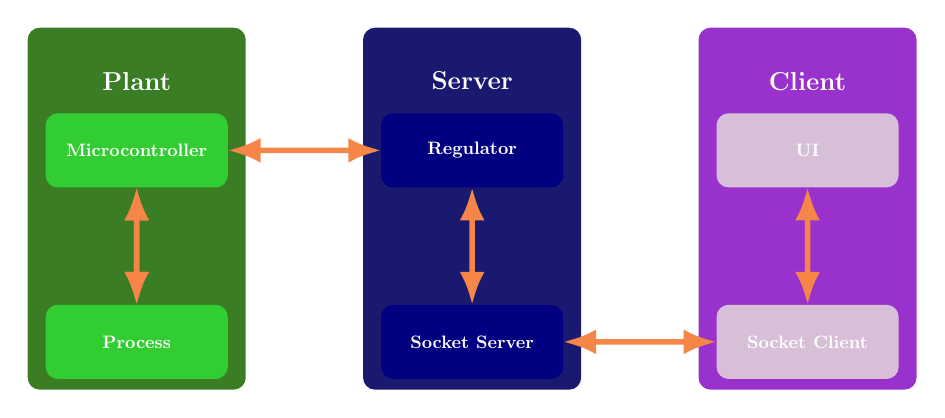
\begin{tikzpicture}[thick, scale=0.65, every node/.style={scale=0.65}]
    \node[draw=OliveGreen, rectangle, minimum width=120, minimum height=200,
    label={[label distance=-180, font=\Large\bf, color=white]-90:Plant},
    fill=OliveGreen, rounded corners]
    (plant) {};

    \node[draw=MidnightBlue, rectangle, minimum width=120, minimum height=200,
    label={[label distance=-180, font=\Large\bf, color=white]-90:Server},
    fill=MidnightBlue, rounded corners, right=1.5 of plant]
    (daemon) {};

    \node[draw=DarkOrchid, rectangle, minimum width=120, minimum height=200,
    label={[label distance=-180, font=\Large\bf, color=white]-90:Client},
    fill=DarkOrchid, rounded corners, right=1.5 of daemon]
    (client) {};

    \node[draw=LimeGreen, rectangle, rounded corners, minimum height=40,
          minimum width=100, fill=LimeGreen, below=-3.5 of plant, font=\bf]
          (arduino) {\textcolor{white}{Microcontroller}};

    \node[draw=LimeGreen, rectangle, rounded corners, minimum height=40,
          minimum width=100, fill=LimeGreen, below=1.5 of arduino, font=\bf]
          (process) {\textcolor{white}{Process}};

    \node[draw=NavyBlue, rectangle, rounded corners, minimum height=40,
          minimum width=100, fill=NavyBlue, below=-3.5 of daemon, font=\bf]
          (regulator) {\textcolor{white}{Regulator}};

    \node[draw=NavyBlue, rectangle, rounded corners, minimum height=40,
          minimum width=100, fill=NavyBlue, below=1.5 of regulator, font=\bf]
          (sserver) {\textcolor{white}{Socket Server}};

    \node[draw=Thistle, rectangle, rounded corners, minimum height=40,
          minimum width=100, fill=Thistle, below=-3.5 of client, font=\bf]
          (UI) {\textcolor{white}{UI}};

    \node[draw=Thistle, rectangle, rounded corners, minimum height=40,
          minimum width=100, fill=Thistle, below=1.5 of UI, font=\bf]
          (sclient) {\textcolor{white}{Socket Client}};

    \draw[Latex-Latex, line width=2, color=Peach] (arduino) to (regulator);
    \draw[Latex-Latex, line width=2, color=Peach] (arduino) to (process);
    \draw[Latex-Latex, line width=2, color=Peach] (arduino) to (process);
    \draw[Latex-Latex, line width=2, color=Peach] (sserver) to (sclient);
    \draw[Latex-Latex, line width=2, color=Peach] (regulator) to (sserver);
    \draw[Latex-Latex, line width=2, color=Peach] (UI) to (sclient);
\end{tikzpicture}
\label{fig:main_sheme}
\end{figure}
\end{frame}

\begin{frame}[fragile]
    \frametitle{Postrojenje}
    \begin{figure}[H]
    \centering
    \includegraphics{../figures/arduino_uno.pdf}
    \label{fig:arduino}
    \end{figure}
\end{frame}

\begin{frame}[fragile]
    \frametitle{Server}
    \begin{figure}[H]
    \centering
    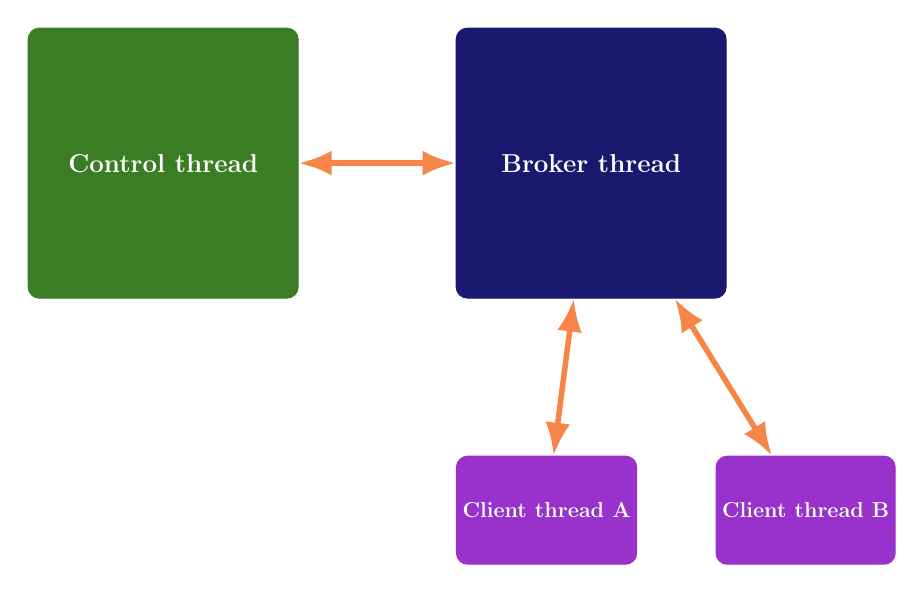
\begin{tikzpicture}[scale=0.65, every node/.style = {font=\Large\bf, scale=0.65},
                        connection/.style = {Latex-Latex, Peach, line width=2}]
        \node[draw=OliveGreen,rectangle, rounded corners,
              fill=OliveGreen, minimum size=150]
              (regulator) {\textcolor{white}{Control thread}};

        \node[draw=MidnightBlue, rectangle, rounded corners, minimum size=150,
              right=2cm of regulator, fill=MidnightBlue]
              (server) {\textcolor{white}{Broker thread}};

        \node[draw=DarkOrchid, rectangle, rounded corners,
              minimum size=60, below left=2cm and -2.3cm of server, font=\bf\large,
              fill=DarkOrchid]
              (clientA) {\textcolor{white}{Client thread A}};

        \node[draw=DarkOrchid, rectangle, rounded corners,
              minimum size=60, right=of clientA, font=\bf\large,
              fill=DarkOrchid]
              (clientB) {\textcolor{white}{Client thread B}};

        \draw[connection] (regulator) to (server);
        \draw[connection] (server)    to (clientA);
        \draw[connection] (server)    to (clientB);
    \end{tikzpicture}
    \label{fig:architecture}
    \end{figure}
\end{frame}

\begin{frame}[fragile]
    \frametitle{Klijent}
    \begin{figure}[H]
    \centering
    \includegraphics[scale=0.15]{../figures/arclient-2.png}
    \label{fig:arduino}
    \end{figure}
\end{frame}

\plain{Demo.}

\plain{Hvala na pažnji.}

\end{document}
